\chapter{Introduction}

% Software aging: https://www.cs.drexel.edu/~yfcai/CS451/RequiredReadings/SoftwareAging.pdf
% Measuring and Monitoring Technical Debt http://ccsl.org.br/files/TD%20talk%20USP.pdf

Quality assurance (QA) is an easily overlooked process in many companies. A mature and well-designed quality assurance system increases customer satisfaction, credibility of the company and optimizes development flows. Solid QA is a fundamental and necessary step in every respectable software engineering project.\\\\
Failure to maintain a proper quality assurance program can lead to catastrophic disasters. On January 28, 1986, The Space Shuttle Challenger, part of NASA's space program, exploded, destroying the vehicle and killing several crew members. This accident was caused by a hardware failure of a solid rocket booster. Several severe flaws in quality assurance and human decision making contributed to this event.\\\\
The importance of quality assurance is also present outside field of the software engineering. Toyota Motor Corp. recalled 3.8 million vehicles in 2009 due to problems with a removable floor mat that could cause accelerators to get stuck. This issue can cause a crash, serious injuries or even death. Again, with right quality assurance processes and high standards, this recall might have been prevented.\\\\
Well-tested and code of high quality is of uttermost important in the financial world. Software bugs in financial transaction systems can cause customers to lose money.
% https://blog.ethereum.org/2016/06/17/critical-update-re-dao-vulnerability/
On June 17, 2016, Etherium, a blockchain-based decentralized platform for applications, reported a vulnerability in their code, allowing an attacker to steal small sums of cryptocurrency. In 2015, The Rabobank, one of the biggest banks in the Netherlands, released a completely redesigned mobile application. The user experience of the new application was very poor: users reported the application as unusable and many users are delaying the update. Incidents like this have led to leaving customers and a decay in the credibility of the affected companies. This shows the importance of proper testing, code review processes and quality assurance infrastructures.\\\\

\begin{figure}[!h]
	\centering
	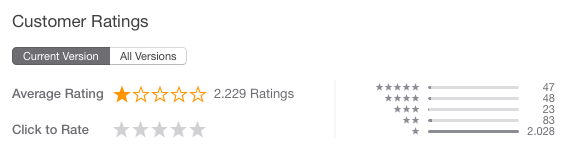
\includegraphics[width=0.6\columnwidth]{images/rabobank_ratings}
	\caption{Reviews of the Rabobank mobile banking app in the App Store.}
	\label{fig:rabobank_reviews}
\end{figure}

When software is developed, the entire development cycle, from design to deployment, is involved with quality assurance. This includes software design, code reviews, testing, version control systems, release management and customer interaction. Quality assurance impacts the user experience.
%[https://www.nngroup.com/articles/quality-assurance-ux/]
When things don't work out for users as expected, users get frustrated and might perform inefficient workarounds. By testing the final product as early as possible, many problems can be fixed already before releasing.\\\\

\begin{figure}[!h]
	\centering
	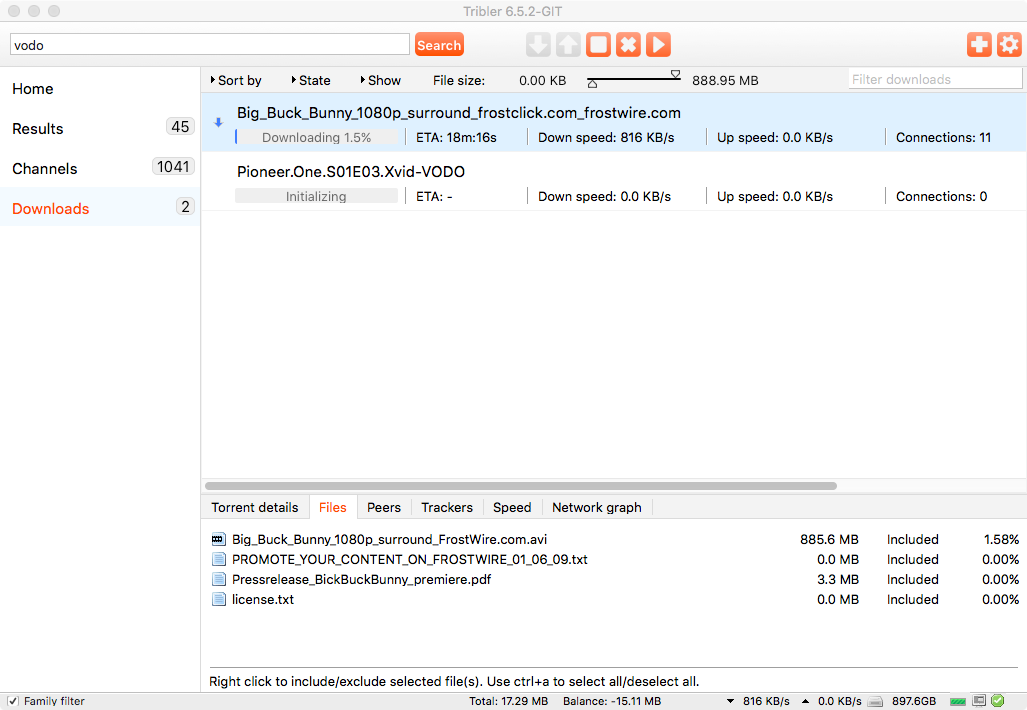
\includegraphics[width=0.9\columnwidth]{images/tribler_interface}
	\caption{The interface of Tribler v6.5.2.}
	\label{fig:tribler_interface}
\end{figure}

This thesis will focus on the quality assurance of a research-oriented prototype named Tribler. Tribler is the result of 10 ongoing years of scientific research. The software allows users to discover and download interesting content such as music and videos. Tribler is built upon the \emph{libtorrent} library and uses a decentralized overlay network to synchronize content between peers. In 2014, support for anonymous download using a Tor-like protocol has been added. In 2015, support for hidden seeding has been added.\\\\
The content of this thesis is structured as follows. The first chapter (linkje) explains ............
